\documentclass[a4paper,11pt]{article} 
\addtolength{\hoffset}{-2.25cm}
\addtolength{\textwidth}{4.5cm}
\addtolength{\voffset}{-3.25cm}
\addtolength{\textheight}{5cm}
\setlength{\parskip}{0pt}
\setlength{\parindent}{0in}

\usepackage[square,sort,comma,numbers]{natbib}
\usepackage{blindtext} % Package to generate dummy text
\usepackage{charter} % Use the Charter font
\usepackage[utf8]{inputenc} % Use UTF-8 encoding
\usepackage{microtype} % Slightly tweak font spacing for aesthetics
\usepackage{amsthm, amsmath, amssymb, amsfonts} % Mathematical typesetting
\usepackage{float} % Improved interface for floating objects
\usepackage{hyperref} % For hyperlinks in the PDF
\usepackage{graphicx, multicol} % Enhanced support for graphics
\usepackage{xcolor} % Driver-independent color extensions
\usepackage{pseudocode} % Environment for specifying algorithms in a natural way
\usepackage[ddmmyy]{datetime} % Uses YEAR-MONTH-DAY format for dates
\usepackage{tikz}
\usepackage{listings}
\usepackage{subcaption}
\usepackage{fancyhdr} % Headers and footers
\pagestyle{fancy} % All pages have headers and footers
\fancyhead{}\renewcommand{\headrulewidth}{0pt} % Blank out the default header
\fancyfoot[L]{} % Custom footer text
\fancyfoot[C]{} % Custom footer text
\fancyfoot[R]{\thepage} % Custom footer text
\newcommand{\note}[1]{\marginpar{\scriptsize \textcolor{red}{#1}}} % Enables comments in red on margin

\DeclareMathOperator*{\argmin}{arg\,min}

\newcount\myloopcounter

\definecolor{codegreen}{rgb}{0,0.6,0}
\definecolor{codegray}{rgb}{0.5,0.5,0.5}
\definecolor{codepurple}{rgb}{0.58,0,0.82}
\definecolor{backcolour}{rgb}{0.95,0.95,0.92}

\lstdefinestyle{mystyle}{
    backgroundcolor=\color{backcolour},   
    commentstyle=\color{codegreen},
    keywordstyle=\color{magenta},
    numberstyle=\tiny\color{codegray},
    stringstyle=\color{codepurple},
    basicstyle=\ttfamily\footnotesize,
    breakatwhitespace=false,         
    breaklines=true,                 
    captionpos=b,                    
    keepspaces=true,                 
    numbers=left,                    
    numbersep=5pt,                  
    showspaces=false,                
    showstringspaces=false,
    showtabs=false,                  
    tabsize=2
}
\lstset{style=mystyle}
%----------------------------------------------------------------------------------------


%-------------------------------
%	TITLE VARIABLES (identify your work!)
%-------------------------------

\newcommand{\yourname}{HUANG Kunlun 57878689} % replace YOURNAME with your name
\newcommand{\youremail}{kl.h@my.cityu.edu.hk} % replace YOUREMAIL with your email
\newcommand{\assignmentnumber}{CS5293 Assignment II} % replace X with the lab session number

\begin{document}

%-------------------------------
%	TITLE SECTION (do not modify unless you really need to)
%-------------------------------
\fancyhead[C]{}
\hrule \medskip
\begin{minipage}{0.295\textwidth} 
\raggedright
\footnotesize
\yourname \hfill\\
\youremail
\end{minipage}
\begin{minipage}{0.4\textwidth} 
\centering 
\large 
Report for \assignmentnumber\\ 
\normalsize 

\end{minipage}
\begin{minipage}{0.295\textwidth} 
\raggedleft
\today\hfill\\
\end{minipage}
\medskip\hrule 
\bigskip


{\hypersetup{hidelinks}
\tableofcontents
}
\newpage
%-------------------------------
%	ASSIGNMENT CONTENT (add your responses)
%-------------------------------
\section{Introduction}
This is the solvement for the CS5293 Assignment II. Each Task have a short statment for the result as well as the procedures or the screenshoot or code listing attached.

\section{Environment Variable and Set-UID Program}

\subsection{Manipulating environment variables}\label{sec:task1}

For this question, 

1. No output occurred when searching for \verb|foo| initially, indicating the variable wasn't part of the environment.

2. After setting \verb|foo| with a string value, it still didn't appear in the environment, as assignment alone doesn't export it.

3. Post \verb|export foo|, the variable \verb|foo| displayed with \verb|printenv|, confirming its addition to the environment.

4. Following \verb|unset foo|, the variable \verb|foo| ceased to appear, signifying its removal from the environment, figured as \ref{fig:task1.2}. 

\begin{figure}[h]
    \centering
  \subfloat[printenv\label{fig:task1.1}]{%
       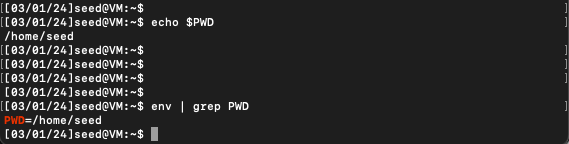
\includegraphics[width=0.35\textwidth]{figures/task1/task1.1.png}}
    \hfill
  \subfloat[set and unset env\label{fig:task1.2}]{%
        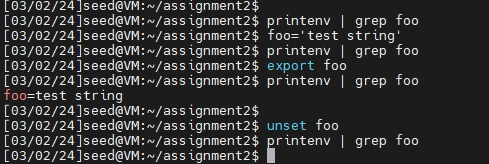
\includegraphics[width=0.54\textwidth]{figures/task1/task1.2.png}}
    \hfill
    \caption{Execute Result}\label{fig:task1}
\end{figure}

\textbf{Conclusion:}

Variables must be exported to appear in the environment. The `unset` command effectively removes them. This demonstrates the lifecycle of environment variables in Bash.

\subsection{Environment variable and Set-UID Programs}

Initially, \verb|foo| was unset and, as expected, didn't appear in the output of the Set-UID program. Upon setting \verb|foo| with a value but without exporting, \verb|foo| still did not show up. This is because the Set-UID program inherits only exported environment variables. After exporting \verb|foo|, it was then visible in the output, indicating that the Set-UID program did inherit \verb|foo| from the user's process as \ref{fig:task2}. 

\begin{figure}[h]
    \centering
       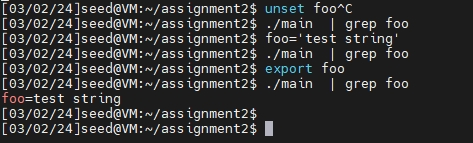
\includegraphics[width=0.7\textwidth]{figures/task2/task2.png}
    \caption{Execute Result}\label{fig:task2}
\end{figure}

\textbf{Conclusion:}

The Set-UID programs inherit exported environment variables from the user's process. This demonstrates how users can influence Set-UID program behavior through the environment, emphasizing the need for careful security practices around such programs.

\subsection{The PATH Environment variable and Set-UID Programs}

The manipulations with the \verb|PATH| variable and the Set-UID \verb|ls| program demonstrate how the system's behavior changed. Initially, the custom \verb|ls| program, when executed, listed the contents of the current directory, similar to the standard \verb|/bin/ls| command. After modifying the \verb|PATH| variable to include the current directory at the beginning and changing the ownership and permissions of the \verb|ls| program to mimic a Set-UID program, the \verb|ls| command should have executed the malicious program. However, the output indicates that the custom \verb|ls| program printed a message and the user IDs, which were both 1000, meaning it did not run with root privileges.

\begin{figure}[h]
    \centering
       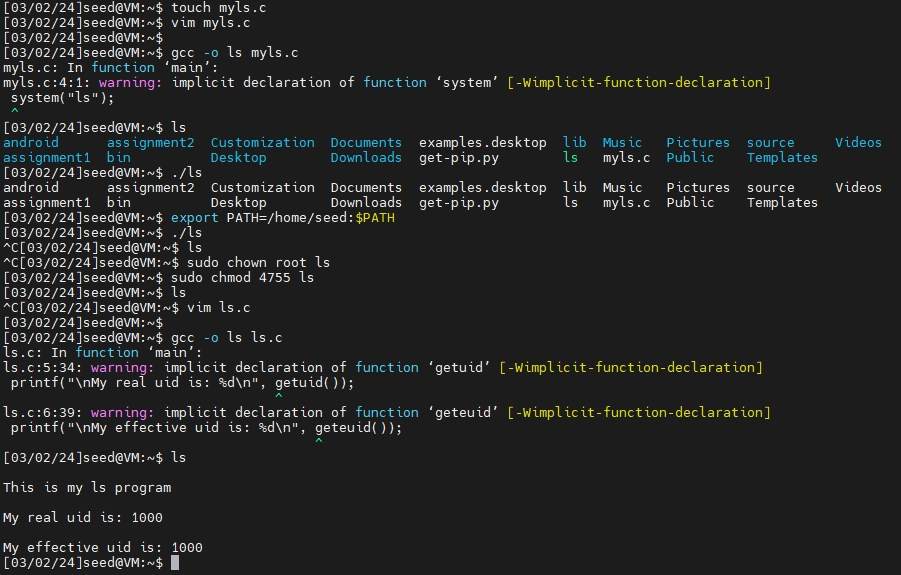
\includegraphics[width=0.95\textwidth]{figures/task3/task3.png}
    \caption{Execute Result}\label{fig:task3}
\end{figure}
\begin{figure}[h]
    \centering
       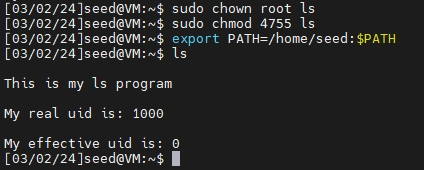
\includegraphics[width=0.5\textwidth]{figures/task3/task3.1.png}
    \caption{Execute Result After Set-UID}\label{fig:task3.1}
\end{figure}

\textbf{Conclusion:}

If the Set-UID program runs our code instead of the intended \verb|/bin/ls|, the code will execute with root privileges because Set-UID programs run with the effective permissions of the file owner, which is root in this case. This demonstrates a significant security risk with using relative paths in Set-UID programs and highlights the importance of using absolute paths for system calls.

\subsection{The LD\_PRELOAD environment variable and Set-UID Programs}
1. When \verb|myprog| was a regular program, running it as a normal user resulted in the overridden \verb|sleep| function being called, confirming that \verb|LD_PRELOAD| influenced the linker to load \verb|libmylib.so.1.0.1| first.

2. After making \verb|myprog| a Set-UID root program, running it as a normal user did not invoke the overridden \verb|sleep|, indicating that the Set-UID program did not inherit the \verb|LD_PRELOAD| variable from the user's environment, likely for security reasons.

3. Exporting \verb|LD_PRELOAD| in the root account and then running the Set-UID root \verb|myprog| resulted in the overridden \verb|sleep| being called, suggesting that when the Set-UID program is run by root, it respects the \verb|LD_PRELOAD| variable.

4. With \verb|myprog| set as a Set-UID program owned by another user (user1) and \verb|LD_PRELOAD| set in a non-root account, the overridden \verb|sleep| was not called, similar to the second case, reinforcing the idea that Set-UID programs ignore \verb|LD_PRELOAD| from non-owner environments.

\begin{figure}[h]
    \centering
       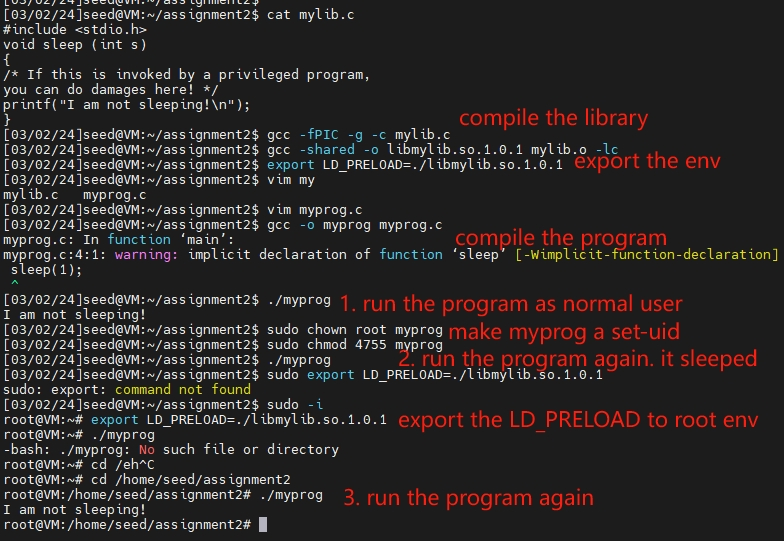
\includegraphics[width=0.9\textwidth]{figures/task4/task4.png}
    \caption{Execute Result}\label{fig:task4}
\end{figure}

\subsection{Invoking external programs using system() versus execve()}
1.If Bob were to exploit the \verb|system()| call with a command like ``./25 /etc/passwd; rm -f /path/to/some/file", as figured in \ref{fig:task5.1}, the shell would execute the \verb|cat /etc/passwd| command and then attempt the \verb|rm -f| command, potentially allowing unauthorized file deletion if the syntax were correct and the shell executes the second command.

The use of \verb|system()| in a Set-UID program poses a security risk due to its reliance on the shell, which can interpret additional commands and metacharacters. This risk is not present with \verb|execve()| as it does not invoke a shell and executes the specified command directly. The observations suggest that the program is functioning with elevated privileges, but the specific access to \verb|/etc/shadow| could not be confirmed from the provided output.

2.After recompiling and setting the program to use \verb|execve()|, any attempts to use command chaining or injection as part of the input to the Set-UID program should fail, as figured in \ref{fig:task5.2}, input such as \verb|filename; rm -f somefile| would not cause the deletion of \verb|somefile| because \verb|execve()| would attempt to pass the entire string as a single argument to \verb|/bin/cat|, which would then result in an error as it would be an invalid file name.
\begin{figure}[h]
    \centering
  \subfloat[Step 1 Execute Result\label{fig:task5.1}]{%
       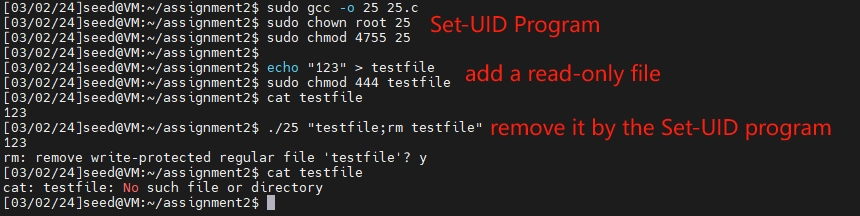
\includegraphics[width=0.95\textwidth]{figures/task5/task5.1.png}}
    \hfill
  \subfloat[Step 2 Execute Result\label{fig:task5.2}]{%
        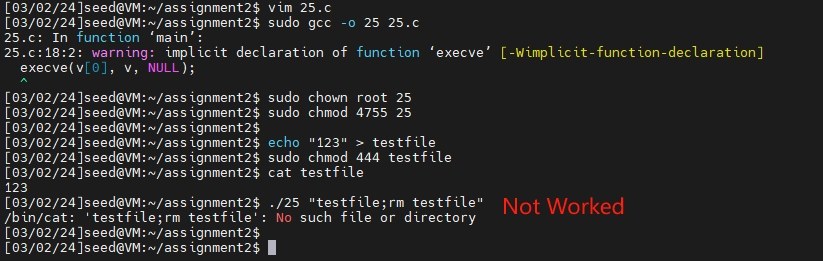
\includegraphics[width=0.95\textwidth]{figures/task5/task5.2.png}}
    \hfill
    \caption{Execute Result}\label{fig:task5}
\end{figure}



\subsection{Capability Leaking}
The program \verb|./26| successfully wrote "Malicious Data" to \verb|/etc/zzz|. Initially unable to open \verb|/etc/zzz|, after setting correct permissions and ownership, the Set-UID program, running with root privileges, opened \verb|/etc/zzz|. Upon dropping privileges with \verb|setuid(getuid())|, the child process inherited the file descriptor with root access, leading to the capability leak which allowed writing to the file, even as a non-privileged user. This demonstrates the security risk of inheriting file descriptors from privileged processes.

\begin{figure}[h]
    \centering
       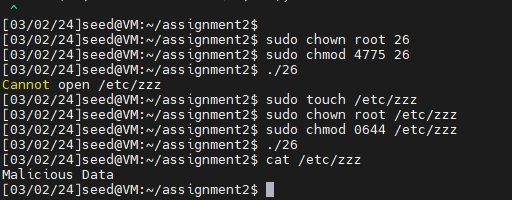
\includegraphics[width=0.7\textwidth]{figures/task6/task6.png}
    \caption{Execute Result}\label{fig:task6}
\end{figure}

\section{Buffer Overflow Vulnerability}

\subsection{Initial setup}

\begin{lstlisting}[caption={CMD},label={lst:task2.7},language=BASH,breaklines=true]
# The provided steps for buffer overflow vulnerability exploitation:
# 1. Disable address space layout randomization (ASLR) which makes address guessing difficult:
sudo sysctl -w kernel.randomize_va_space=0
# 2. Compile programs without the StackGuard protection to allow buffer overflow attacks:
gcc -fno-stack-protector example.c
# 3. By default, Ubuntu stacks are non-executable. To ensure stack executability is not a factor, compile programs with non-executable stack protection:
gcc -z noexecstack -o test test.c
# 4. Change the `/bin/sh` symbolic link to point to a shell without Set-UID restrictions like `zsh` (only for Ubuntu 16.04 as it has countermeasures in `dash`):
sudo ln -sf /bin/zsh /bin/sh
\end{lstlisting} 

Disabling ASLR makes buffer overflow attacks easier by making memory addresses predictable. ASLR randomizes locations of the stack, heap, and libraries, complicating an attacker's ability to correctly guess where to inject malicious code or overwrite a return address. Without ASLR, these addresses remain constant, so attackers can reliably target specific memory locations to execute their code, significantly increasing the chances of a successful attack.

\begin{figure}[h]
    \centering
       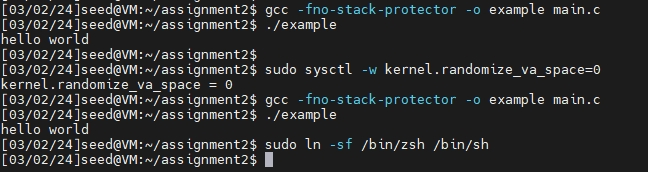
\includegraphics[width=0.8\textwidth]{figures/task7/task7.png}
    \caption{Execute Result}\label{fig:task7}
\end{figure}


\subsection{Running Shellcode}

As shown in Figure \ref{fig:task8.1}, the commands compile and run \verb|shell.c|, which launches a shell. Initially, running \verb|./shell| as the user \verb|seed| opens a shell with user-level privileges. After setting the program's owner to root and adding the Set-UID bit, running \verb|./shell| again opens a shell with root privileges, confirmed by the output of \verb|whoami|. This demonstrates how a Set-UID root-owned program can elevate privileges, highlighting the potential for exploitation if such a program were vulnerable to a buffer overflow attack, allowing unauthorized execution of code with elevated rights.

\begin{figure}[h]
    \centering
       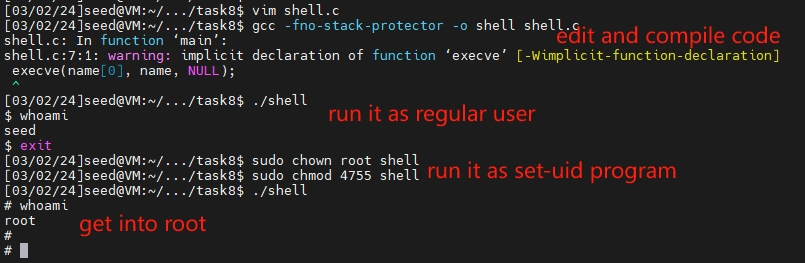
\includegraphics[width=0.8\textwidth]{figures/task8/task8.1.png}
    \caption{Execute Result}\label{fig:task8.1}
\end{figure}

As shown in Figure \ref{fig:task8.2}, When compiled with executable stack permission \verb|-z execstack| and run as a normal user, the program launches a shell with user-level privileges \verb|seed|. After changing the ownership to root and setting the Set-UID bit \verb|chmod 4755`|, the same program now launches a shell with root privileges, as the effective UID of the process is escalated due to the Set-UID bit. This illustrates a potential security threat when executable code is present in the stack, especially in Set-UID programs.
\begin{figure}[h]
    \centering
       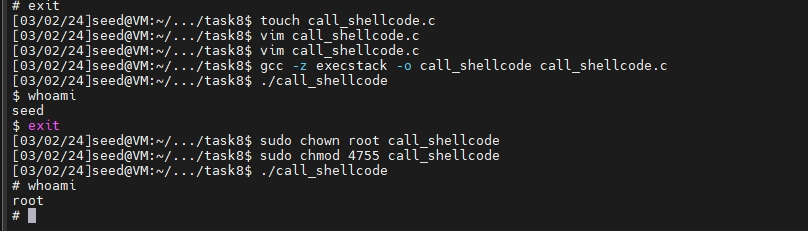
\includegraphics[width=0.8\textwidth]{figures/task8/task8.2.png}
    \caption{Execute Result}\label{fig:task8.2}
\end{figure}

\subsection{The Vulnerable Program}
The program \verb|stack.c| has a deliberate buffer overflow vulnerability. It reads data from a file named \verb|badfile| into a buffer that can only hold \verb|BUFSIZE| bytes (33 by default) using \verb|strcpy()|, which does not check for buffer overflow. If \verb|badfile| contains more data than \verb|BUFSIZE|, it will overflow the buffer \verb|buffer[BUFSIZE]| in \verb|bof()| function and potentially overwrite adjacent memory, which might include the function's return address.

As shown in Figure \ref{fig:task9}, The segmentation faults when running \verb|./stack| indicate that the program crashes due to a buffer overflow caused by incorrect or corrupted data in \verb|badfile|. This is indicative of the vulnerability, and with the right \verb|badfile| contents, an attacker could leverage this to execute arbitrary code with root privileges.
\begin{figure}[h]
    \centering
       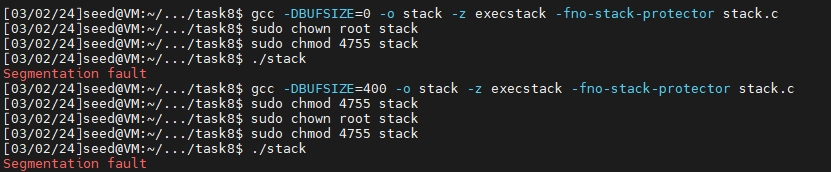
\includegraphics[width=0.8\textwidth]{figures/task9/task9.png}
    \caption{Execute Result}\label{fig:task9}
\end{figure}

\subsection{Exploiting the Vulnerability}
First, GDB debug for the stack, find out the \verb|bof| and \verb|strcpy| addresses, figured as \ref{fig:task10.1} and figured as \ref{fig:task10.2}, respectively.
\begin{lstlisting}[caption={GDB debug for the stack},label={lst:task3.10-1},language=BASH,breaklines=true]
gdb stack
disas main
disas bof
\end{lstlisting} 

\begin{figure}[h]
    \centering
  \subfloat[bof address\label{fig:task10.1}]{%
       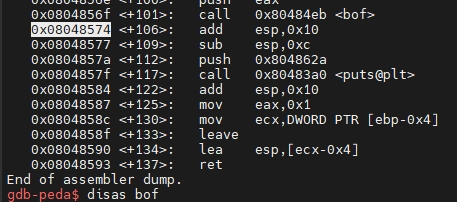
\includegraphics[width=0.49\textwidth]{figures/task10/task10.1.png}}
    \hfill
  \subfloat[strcpy address\label{fig:task10.2}]{%
        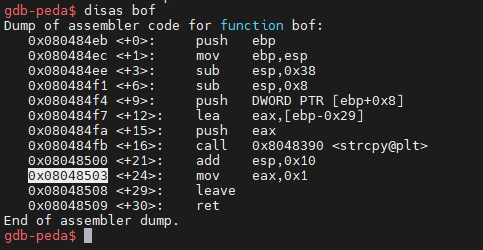
\includegraphics[width=0.49\textwidth]{figures/task10/task10.2.png}}
    \hfill
    \caption{GDB debug for the stack}\label{fig:task10-1}
\end{figure}

then, edit the \verb|exploit.c| as Codeblock \ref{lst:task3.10-2} and run the GDB again figured as \ref{fig:task10-2} for figuring out the memory length.
\begin{lstlisting}[caption={GDB debug for the stack},label={lst:task3.10-2},language=C,breaklines=true]
/* You need to fill the buffer with appropriate contents here */
strcpy(buffer, "AAAA");
\end{lstlisting} 

\begin{figure}[h]
    \centering
       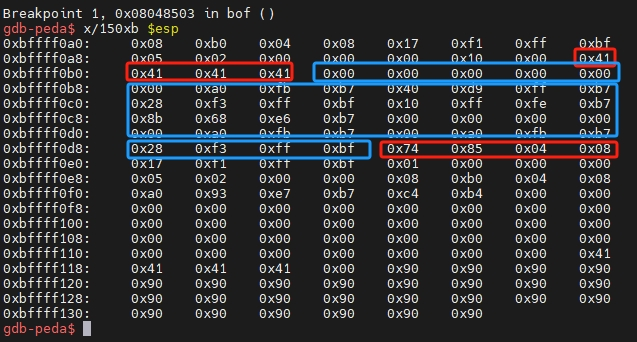
\includegraphics[width=0.7\textwidth]{figures/task10/task10.3.png}
    \caption{Execute Result}\label{fig:task10-2}
\end{figure}

Obviously, we should fill out the buffer with $45$ characters and add a $SHIFT  > 45 + 4$ to the shellcode as Codeblock \ref{lst:task3.10-3}.
\begin{lstlisting}[caption={fill the buffer},label={lst:task3.10-3},language=C,breaklines=true]
/* You need to fill the buffer with appropriate contents here */
strcpy(buffer, "AAAAAAAAAAAAAAAAAAAAAAAAAAAAAAAAAAAAAAAAAAAAA");
strcpy(buffer+50,shellcode);
\end{lstlisting} 

Finally, we compile and run the exploit and stack again, respectively. And we can launch the shell with root privilege, figured as \ref{fig:task10-3}.
\begin{figure}[h]
    \centering
       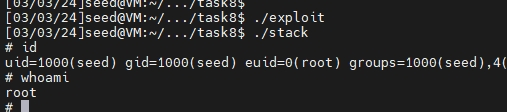
\includegraphics[width=0.7\textwidth]{figures/task10/task10.4.png}
    \caption{Execute Result}\label{fig:task10-3}
\end{figure}

\subsection{Defeating dash’s Countermeasure}

As shown in Figure \ref{fig:task11.1}, When \verb|setuid(0);| is commented out, executing the program as a Set-UID will not grant root privileges because dash drops privileges if the real and effective UIDs differ. Unprivileged commands will confirm the user's identity, not root.

Uncommenting \verb|setuid(0);|, the program elevates privileges by setting the real UID to zero before calling \verb|execve()|, allowing a privileged shell as dash sees matching UIDs. Commands like `whoami` will return \verb|root|, confirming elevated access.

To bypass dash's countermeasure in shellcode, prepend the \verb|setuid(0)| syscall, ensuring the effective UID is set to root before executing privileged operations.
\begin{figure}[h]
    \centering
       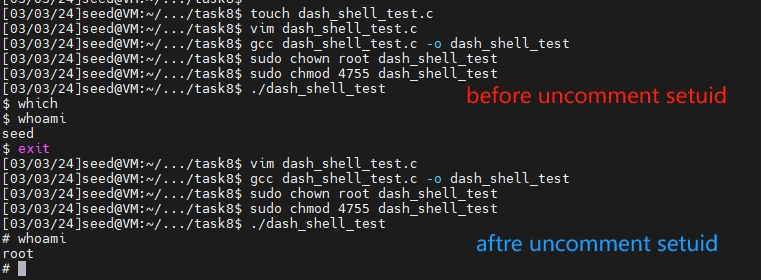
\includegraphics[width=0.8\textwidth]{figures/task11/task11.1.png}
    \caption{Different Behavior}\label{fig:task11.1}
\end{figure}

Figure \ref{fig:task11.2} shows the shellcode in \verb|exploit.c|. This bypasses dash's countermeasure, allowing the Set-UID program to execute with root privileges.
\begin{figure}[h]
    \centering
       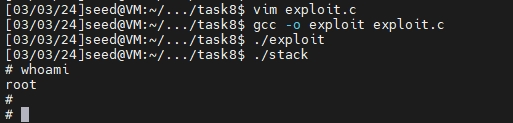
\includegraphics[width=0.8\textwidth]{figures/task11/task11.2.png}
    \caption{Using the above shellcode in exploit.c}\label{fig:task11.2}
\end{figure}

\subsection{Defeating Address Randomization}
With ASLR enabled, the exploit may fail as memory addresses are randomized, making the hardcoded addresses unreliable. The exploit's success becomes unpredictable because the return address might not point to the intended shellcode location.

Running the exploit multiple times might eventually succeed because the randomized addresses could align with the shellcode by chance. A larger NOP sled may increase this likelihood, but success is not guaranteed and can take numerous attempts.

In my experiment, No shell was obtained. The segmentation fault after 1,333,478 attempts, figured as \ref{fig:task12}, indicates the exploit consistently hit invalid memory addresses due to Address Space Layout Randomization (ASLR). ASLR randomizes the location of the stack, heap, and libraries, making it challenging for the exploit to predict where to jump to execute the shellcode. The exploit relies on precise addresses; ASLR's randomization ensures that each execution of the vulnerable program maps the stack differently, preventing the exploit from knowing the correct address to use. Repeated attempts increase the likelihood but do not guarantee success, as demonstrated by the large number of failed tries.
\begin{figure}[h]
    \centering
       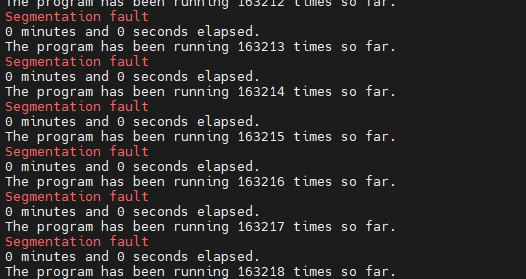
\includegraphics[width=0.6\textwidth]{figures/task12/task12.png}
    \caption{Using the above shellcode in exploit.c}\label{fig:task12}
\end{figure}

\subsection{Stack Guard Protection}
The program \verb|stack| was recompiled without disabling Stack Guard as figured as \ref{fig:task13}. Upon the execution, a buffer overflow attempt was made, and Stack Guard detected the attack, triggering a error message as \verb| *** stack smashing detected ***: ./stack terminated| and aborting the program. 

This error confirms that Stack Guard's canary mechanism effectively prevents buffer overflow by monitoring for stack corruption and stopping execution if tampering is detected. This defense significantly increases the difficulty of exploiting such vulnerabilities.

\begin{figure}[h]
    \centering
       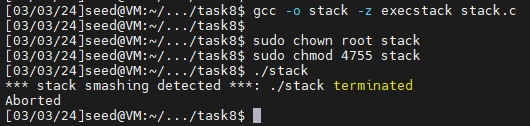
\includegraphics[width=0.7\textwidth]{figures/task13/task13.png}
    \caption{Stack Guard Protection}\label{fig:task13}
\end{figure}

\subsection{Non-executable Stack Protection}
No shell was obtained after recompiling the program with the non-executable stack option as figured as \ref{fig:task14}. The problem is that the stack has been configured to disallow code execution, so even if a buffer overflow occurs and attempts to run shellcode placed on the stack, the CPU will refuse to execute it, leading to a segmentation fault instead. While this protection scheme prevents execution of shellcode on the stack, it does not stop buffer overflows from occurring or other exploitation techniques like Return Oriented Programming (ROP) that can leverage executable code segments elsewhere. The segmentation fault indicates an attempt to execute code on a non-executable stack.
\begin{figure}[h]
    \centering
       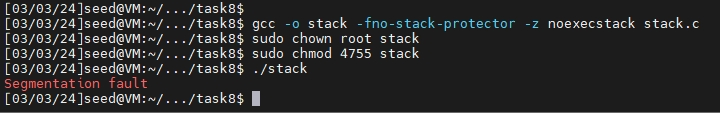
\includegraphics[width=0.7\textwidth]{figures/task14/task14.png}
    \caption{Stack Guard Protection}\label{fig:task14}
\end{figure}

\section{Return-to-libc Attack}
\subsection{Initial Setup}

%------------------------------------------------

%\bibliographystyle{ieeetr}
%\bibliography{references} % citation records are in the references.bib document

\end{document}
